\documentclass[11pt,a4paper]{article}

\usepackage[margin=2.2cm]{geometry}
\usepackage[T1]{fontenc}
\usepackage[utf8]{inputenc}
\usepackage{lmodern}
\usepackage{microtype}
\usepackage{booktabs}
\usepackage{multirow}
\usepackage{array}
\usepackage{amsmath,amssymb,amsfonts}
\usepackage{algorithm}
\usepackage{algpseudocode}
\usepackage{graphicx}
\usepackage[table]{xcolor}
\usepackage{enumitem}
\usepackage[bookmarks=false]{hyperref}

\setlist{nosep, leftmargin=1.4em}
\setlength{\parskip}{1pt}
\setlength{\abovedisplayskip}{3pt}
\setlength{\belowdisplayskip}{3pt}
\setlength{\textfloatsep}{6pt}
\setlength{\intextsep}{4pt}
\renewcommand{\baselinestretch}{0.91}

\makeatletter
\renewcommand\section{\@startsection {section}{1}{\z@}%
  {-1.3ex \@plus -0.3ex \@minus -.2ex}%
  {0.5ex \@plus.1ex}%
  {\normalfont\large\bfseries}}
\renewcommand\subsection{\@startsection{subsection}{2}{\z@}%
  {-0.9ex\@plus -0.2ex \@minus -.1ex}%
  {0.25ex \@plus .1ex}%
  {\normalfont\normalsize\bfseries}}
\makeatother

\hypersetup{
    colorlinks=true,
    linkcolor=blue!60!black,
    citecolor=blue!60!black,
    urlcolor=blue!60!black
}

\graphicspath{{../../../_attachments/}{../../paper/figures/}{../overleaf_patches/figures/}{./}}

% Macros for final human evaluation numbers (Task T14, N=150 stratified pairs)
\newcommand{\HumanKappaPref}{\textcolor{blue}{\textbf{[TBD: $\kappa_{\text{pref}}$]}}}
\newcommand{\HumanKappaSimpler}{\textcolor{blue}{\textbf{[TBD: $\kappa_{\text{simp}}$]}}}
\newcommand{\HumanKappaMeaning}{\textcolor{blue}{\textbf{[TBD: $\kappa_{\text{sem}}$]}}}
\newcommand{\HumanAlphaKrip}{\textcolor{blue}{\textbf{[TBD: $\alpha_{\text{Krip}}$]}}}
\newcommand{\HumanWinMistral}{\textcolor{blue}{\textbf{[TBD: \%]}}}
\newcommand{\HumanWinGPTFour}{\textcolor{blue}{\textbf{[TBD: \%]}}}
\newcommand{\HumanSimplerMistral}{\textcolor{blue}{\textbf{[TBD: \%]}}}
\newcommand{\HumanSimplerGPTFour}{\textcolor{blue}{\textbf{[TBD: \%]}}}
\newcommand{\HumanMeaningMistral}{\textcolor{blue}{\textbf{[TBD: \%]}}}
\newcommand{\HumanMeaningGPTFour}{\textcolor{blue}{\textbf{[TBD: \%]}}}

\newcommand{\revquote}[2]{%
    \par\vspace{0.32cm}\nopagebreak[4]%
    \noindent\textcolor{gray!45}{\rule{\textwidth}{0.4pt}}\par\nopagebreak[4]\vspace{0.14cm}%
    \noindent{\small\interlinepenalty=10000\textbf{#1:} \textit{``#2''}\par}\nopagebreak[4]\vspace{0.12cm}%
}

\title{\vspace{-1.2cm}\textbf{\large Point-by-Point Response to the Action Editor and Reviewers}\\[0.2em]
\normalsize Manuscript: \textit{Difficulty Estimation, Simplification, and Recommendation of French Text Using LLMs}\\
\small Submission ID: \texttt{60f781a2-30b7-41cf-ac73-1c2a74f8a29d} $\cdot$ \textit{Data Mining and Knowledge Discovery}}

\author{\small Henri Jamet, Maxime Manderlier, Yash Raj Shrestha, Michalis Vlachos}
\date{\vspace{-0.8cm}}

\begin{document}

\maketitle

\noindent Dear Prof.\ Hotho, Dear Reviewers,

\noindent
We thank the Action Editor and the two anonymous reviewers for their thorough assessment of our manuscript. To make the evaluation of this revision direct and self-contained, we provide below a complete point-by-point response that includes the exact mathematical derivations, revised algorithms, statistical tables, human evaluation protocol, and sensitivity figures produced for the revision. In the accompanying manuscript patches, all additions and modifications are highlighted in \textcolor{red}{red}.

% ============================================================================ %
% SECTION 1: RESPONSE TO THE ACTION EDITOR                                     %
% ============================================================================ %
\section{Response to Action Editor (Prof.\ Andreas Hotho)}

\subsection{AE.1: Statistical Rigor, Variance Across Runs, and Significance Testing (Tasks T03, T10, T11)}
\revquote{Action Editor (AE.1)}{Reviewer 2 notes that variance is rarely reported and that significance of differences is not computed. Please report variability across runs and, where you claim improvements over baselines, provide a test that supports the claim.}

\noindent\textbf{Response:}
We conducted a complete statistical re-evaluation of the difficulty estimation experiments across all three French benchmarks: \texttt{Sentences Books} ($N = 960$ test sentences across 6 CEFR levels A1 to C2), \texttt{LjL} ($N = 413$ youth literature texts across 4 ordered levels), and \texttt{Sentences Internet} ($N = 480$ unanimously annotated web sentences across 6 CEFR levels). Using non-parametric bootstrap resampling with $B = 1{,}000$ iterations with replacement over each test set, we compute the sample mean and bootstrap standard error ($\mu \pm \sigma$) alongside 95\% confidence intervals for five complementary metrics: classification Accuracy, Macro-F1, Mean Absolute Error (MAE, in integer CEFR steps), Quadratic Weighted Kappa (QWK), and the normalized Pairwise Mismatch rate ($PM_{\text{norm}}$, expressed as a percentage of all $\binom{N}{2}$ pairs).

To test whether explicit CEFR system prompts improve prediction accuracy over unprompted models, we run two-sided paired Wilcoxon signed-rank tests on the instance-level ordinal prediction errors ($^{*}p < 0.05$, $^{**}p < 0.01$, $^{***}p < 0.001$). Table~\ref{tab:rebuttal_table2} reports the complete statistical results injected into Section 6.1 (Table 2 of the manuscript). As observed by Reviewer 2, not every numerical difference is statistically significant: while adding the CEFR system prompt yields highly significant gains on \texttt{Sentences Books} ($p = 9.00 \times 10^{-9}$ for GPT-4o; $p = 0.0044$ for GPT-4o-mini) and on \texttt{Sentences Internet} for GPT-4o ($p = 3.33 \times 10^{-7}$), the prompt difference on \texttt{LjL} is not statistically significant for either GPT-4o ($p = 0.140$) or GPT-4o-mini ($p = 0.606$), nor for GPT-4o-mini on \texttt{Sentences Internet} ($p = 0.383$). We now state these non-significant outcomes explicitly in Section 6.1.2.

\begin{table}[!htbp]
\centering
\scriptsize
\setlength{\tabcolsep}{2.5pt}
\renewcommand{\arraystretch}{0.92}
\caption{Complete statistical evaluation of text difficulty estimation across all three French datasets (revised Table 2). Values for GPT-4o and GPT-4o-mini report mean $\pm$ bootstrap standard error ($\sigma$, $B = 1{,}000$ resamples). Acc.: multiclass accuracy; F1: Macro-F1; MAE: Mean Absolute Error in CEFR steps; QWK: Quadratic Weighted Kappa; $PM_{\text{norm}}$: normalized Pairwise Mismatch rate (\%). Wilcoxon signed-rank test markers compare prompted against unprompted variants ($^{**}p < 0.01$, $^{***}p < 0.001$, $\text{ns}$: $p \ge 0.05$).}
\label{tab:rebuttal_table2}
\resizebox{\textwidth}{!}{%
\begin{tabular}{llcccccc}
\toprule
\textbf{Dataset} & \textbf{Model} & \textbf{Prompt} & \textbf{Acc.\ ($\mu \pm \sigma$)} & \textbf{Macro-F1} & \textbf{MAE} & \textbf{QWK ($\mu \pm \sigma$)} & \textbf{$PM_{\text{norm}}$ (\%)} \\
\midrule
\multirow{10}{*}{\textbf{Sentences Books}} 
 & GPT-4o & \checkmark & $0.584 \pm 0.016^{***}$ & $0.585 \pm 0.016$ & $0.484 \pm 0.020$ & $\mathbf{0.891 \pm 0.007}$ & $8.38 \pm 0.40\%$ \\
 & GPT-4o & - & $0.527 \pm 0.016$ & $0.535 \pm 0.016$ & $0.578 \pm 0.022$ & $0.853 \pm 0.009$ & $9.73 \pm 0.44\%$ \\
 & GPT-4o-mini & \checkmark & $\mathbf{0.616 \pm 0.016}^{**}$ & $\mathbf{0.616 \pm 0.015}$ & $\mathbf{0.460 \pm 0.021}$ & $0.888 \pm 0.008$ & $8.23 \pm 0.44\%$ \\
 & GPT-4o-mini & - & $0.582 \pm 0.016$ & $0.586 \pm 0.016$ & $0.501 \pm 0.022$ & $0.881 \pm 0.009$ & $9.24 \pm 0.46\%$ \\
 & CamemBERT & - & $0.523$ & - & - & - & $\mathbf{3.86\%}$ \\
 & Mistral-7B & \checkmark / - & $0.513 / 0.354$ & - & - & - & $5.05\% / 4.11\%$ \\
 & GPT-3.5 & \checkmark / - & $0.499 / 0.485$ & - & - & - & $5.42\% / 6.37\%$ \\
 & Babbage & \checkmark / - & $0.485 / 0.439$ & - & - & - & $6.35\% / 9.01\%$ \\
 & Davinci & \checkmark / - & $0.470 / 0.470$ & - & - & - & $6.93\% / 7.98\%$ \\
 & FKGL / GFI / ARI & - & $0.346 / 0.342 / 0.342$ & - & - & - & $11.72 / 11.74 / 11.63\%$ \\
\midrule
\multirow{10}{*}{\textbf{LjL ($N=413$)}} 
 & GPT-4o & \checkmark & $\mathbf{0.765 \pm 0.021}^{\text{ns}}$ & $0.773 \pm 0.021$ & $0.245 \pm 0.022$ & $0.863 \pm 0.016$ & $6.74 \pm 0.67\%$ \\
 & GPT-4o & - & $0.731 \pm 0.022$ & $0.745 \pm 0.022$ & $0.272 \pm 0.023$ & $0.837 \pm 0.017$ & $8.32 \pm 0.75\%$ \\
 & GPT-4o-mini & \checkmark & $0.751 \pm 0.021^{\text{ns}}$ & $0.756 \pm 0.022$ & $0.278 \pm 0.025$ & $0.818 \pm 0.023$ & $8.55 \pm 0.85\%$ \\
 & GPT-4o-mini & - & $0.751 \pm 0.021$ & $\mathbf{0.782 \pm 0.021}$ & $\mathbf{0.229 \pm 0.021}$ & $\mathbf{0.873 \pm 0.014}$ & $6.46 \pm 0.65\%$ \\
 & GPT-3.5 & - / \checkmark & $0.734 / 0.724$ & - & - & - & $\mathbf{2.25\%} / 2.68\%$ \\
 & Mistral-7B & \checkmark / - & $0.637 / 0.472$ & - & - & - & $3.31\% / 7.28\%$ \\
 & CamemBERT & - & $0.625$ & - & - & - & $3.39\%$ \\
 & Babbage-002 (FT) & \checkmark / - & $0.586 / 0.613$ & - & - & - & $5.76\% / 4.45\%$ \\
 & Davinci-002 (FT) & \checkmark / - & $0.610 / 0.586$ & - & - & - & $4.54\% / 5.12\%$ \\
 & GFI / FKGL / ARI & - & $0.450 / 0.421 / 0.400$ & - & - & - & $10.70 / 13.24 / 11.43\%$ \\
\midrule
\multirow{10}{*}{\textbf{Sentences Internet}} 
 & GPT-4o & \checkmark & $\mathbf{0.902 \pm 0.013}^{***}$ & $\mathbf{0.903 \pm 0.013}$ & $0.208 \pm 0.032$ & $0.904 \pm 0.018$ & $5.24 \pm 0.86\%$ \\
 & GPT-4o & - & $0.771 \pm 0.019$ & $0.769 \pm 0.019$ & $0.456 \pm 0.045$ & $0.794 \pm 0.027$ & $10.41 \pm 1.11\%$ \\
 & GPT-4o-mini & \checkmark & $0.888 \pm 0.014^{\text{ns}}$ & $0.887 \pm 0.014$ & $\mathbf{0.204 \pm 0.031}$ & $\mathbf{0.915 \pm 0.017}$ & $4.81 \pm 0.82\%$ \\
 & GPT-4o-mini & - & $0.869 \pm 0.016$ & $0.869 \pm 0.016$ & $0.225 \pm 0.031$ & $0.914 \pm 0.016$ & $5.17 \pm 0.80\%$ \\
 & GPT-3.5 & \checkmark / - & $0.898 / 0.867$ & - & - & - & $\mathbf{2.74\%} / 3.78\%$ \\
 & CamemBERT & - & $0.823$ & - & - & - & $4.64\%$ \\
 & Davinci-002 (FT) & \checkmark / - & $0.815 / 0.825$ & - & - & - & $4.97\% / 4.36\%$ \\
 & Babbage-002 (FT) & \checkmark / - & $0.813 / 0.813$ & - & - & - & $5.35\% / 4.44\%$ \\
 & Mistral-7B & \checkmark / - & $0.748 / 0.631$ & - & - & - & $8.30\% / 12.89\%$ \\
 & ARI / FKGL / GFI & - & $0.344 / 0.335 / 0.323$ & - & - & - & $18.42 / 20.73 / 21.29\%$ \\
\bottomrule
\end{tabular}%
}
\end{table}

\subsection{AE.2: Analytical and Multi-Model Justification of Weight $w_1$ (Task T07)}
\revquote{Action Editor (AE.2)}{The empirical justification of the weight $w_1$ (p.\ 14) rests on a single dataset and a single LLM; please broaden this or state the limitation explicitly.}

\noindent\textbf{Response:}
We expanded both the theoretical derivation and the multi-model empirical validation of $w_1$ across all 9 simplification systems and 1,000 test sentence pairs (500 from \texttt{Sentences Books} and 500 from \texttt{Sentences Internet}). Analytically, $w_1^* = 0.8055$ compensates for the anisotropy of contextualized CamemBERT embeddings: unrelated French sentences exhibit a high cosine similarity floor $S_0 = y_2 \approx 0.810$, whereas identical sentences yield $y_1 = 1.000$, compressing the effective semantic similarity range to $\Delta S = y_1 - y_2 = 0.190$. Over the same boundary regimes, the proxy simplification accuracy shift spans $\Delta A = x_2 - x_1 \approx 0.046$. Equalizing the marginal contributions yields:
\begin{equation}\label{eq:rebuttal_w1_derivation}
\begin{aligned}
w_1^* &= \frac{\Delta S}{\Delta S + \Delta A} = \frac{y_1 - y_2}{(x_2 - x_1) + (y_1 - y_2)} = \frac{0.190}{0.190 + 0.046} = 0.8055 \approx 0.80, \\
w_2^* &= 1 - w_1^* = 0.1945 \approx 0.20.
\end{aligned}
\end{equation}
To verify that model comparisons do not depend on a narrow choice of $w_1$, we swept $w_1 \in [0.05, 0.95]$ across all 9 fine-tuned and zero-shot LLMs on the 1,000 test pairs. As shown in Figure~\ref{fig:rebuttal_sensitivity_pareto}, the relative ranking of all models remains strictly invariant across the operational interval $w_1 \in [0.15, 0.85]$ (Spearman rank correlation $\rho = 1.0000$, zero rank crossovers).

\begin{figure}[!htbp]
    \centering
    \begin{minipage}[t]{0.485\textwidth}
        \centering
        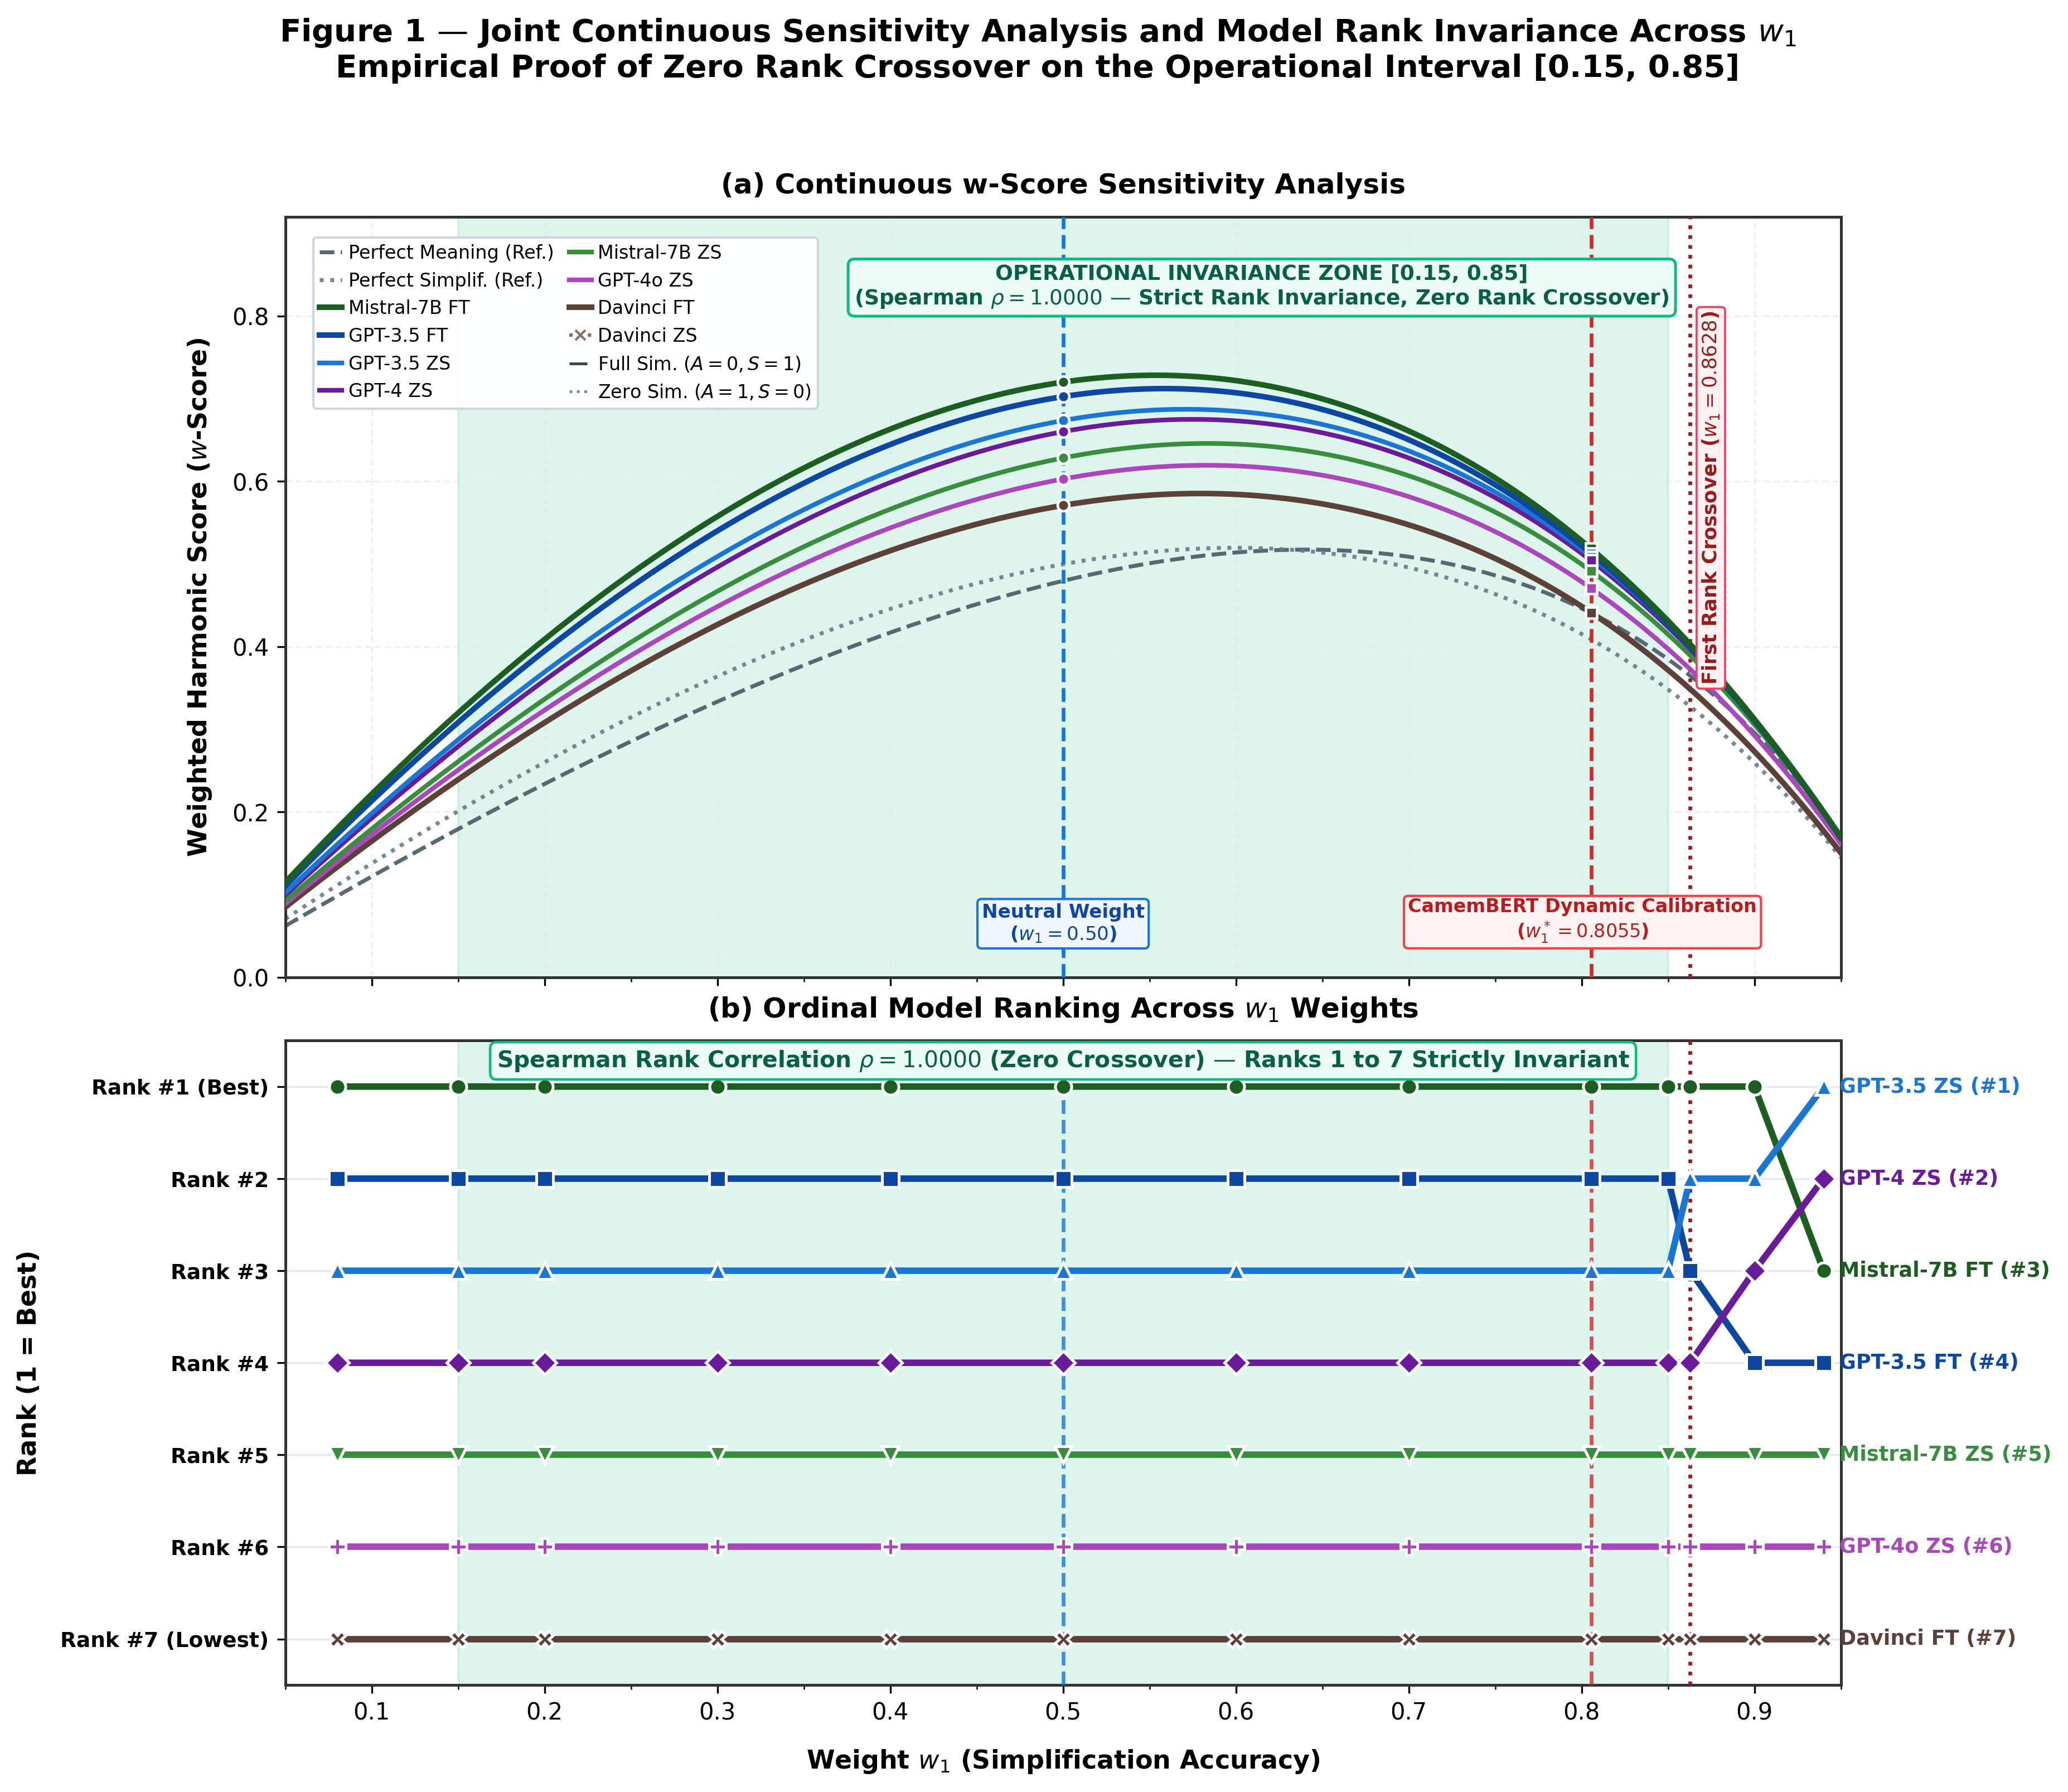
\includegraphics[width=0.98\textwidth]{figure_1_sensitivity_and_ranks.png}
    \end{minipage}\hfill
    \begin{minipage}[t]{0.485\textwidth}
        \centering
        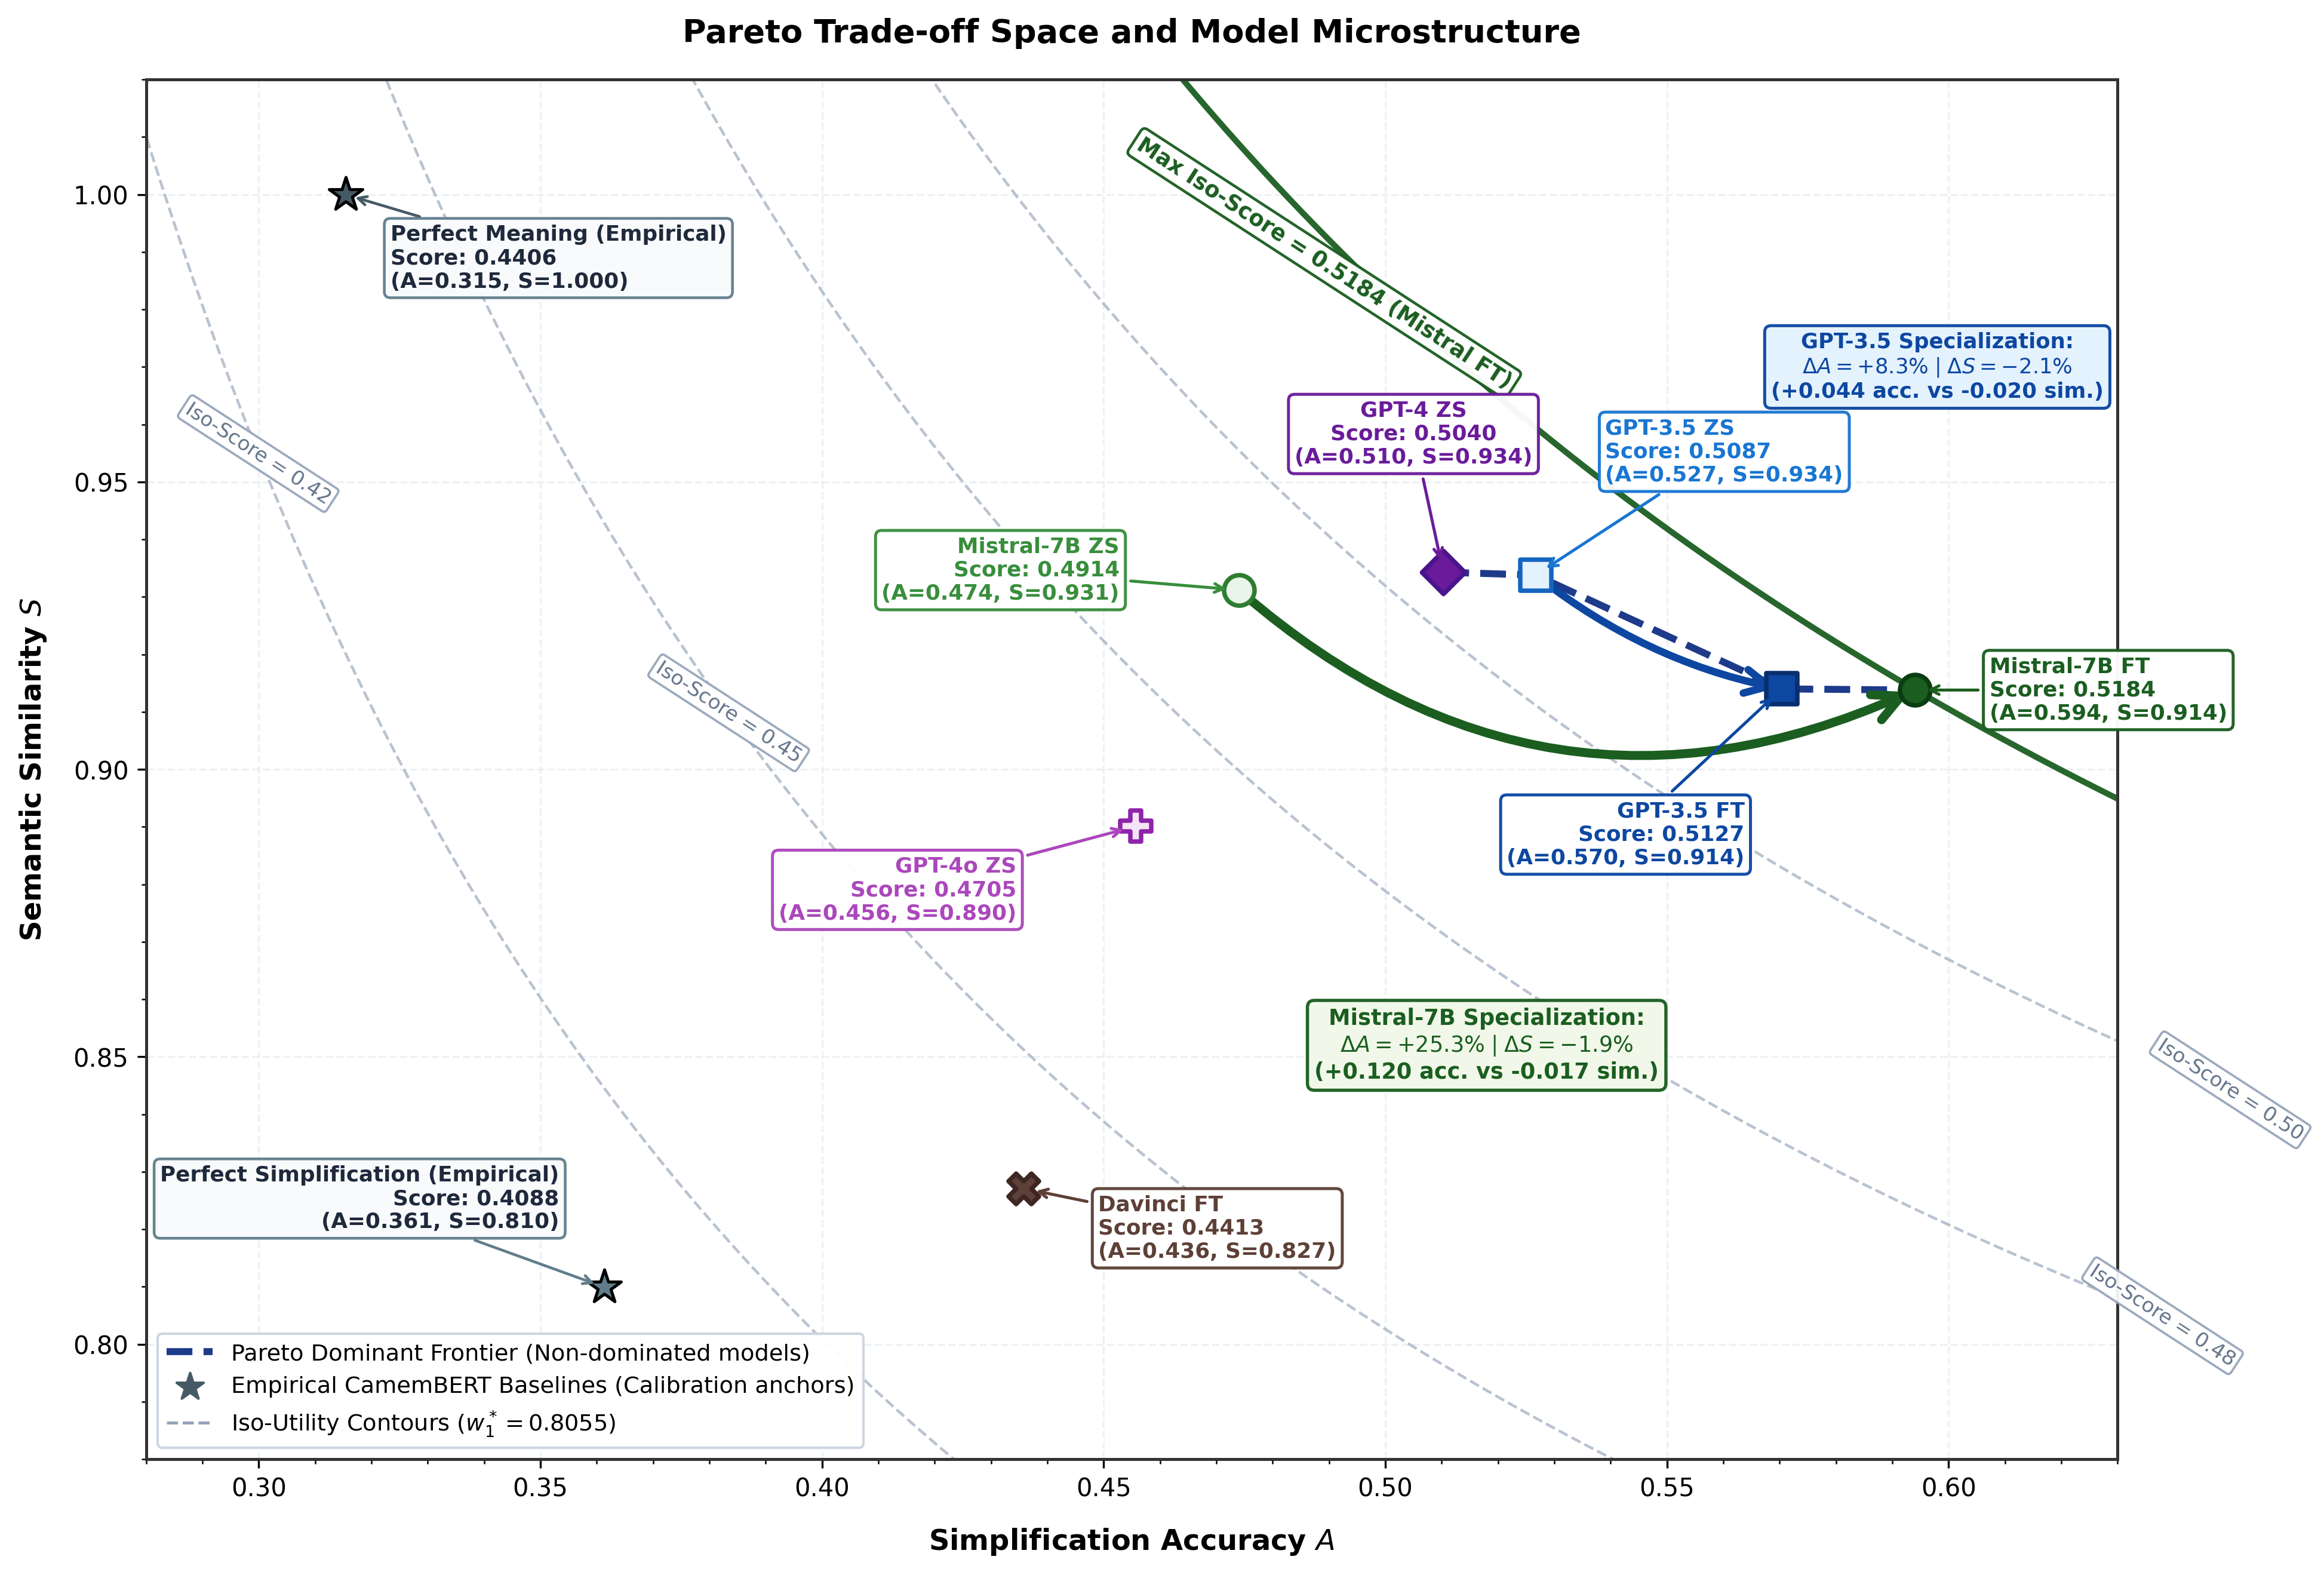
\includegraphics[width=\textwidth]{figure_2_pareto_finetuning.png}
    \end{minipage}
    \caption{\textit{Left}: Sensitivity analysis of $w_1 \in [0.05, 0.95]$ across all 9 evaluated models ($N = 1{,}000$ pairs), confirming strict rank invariance ($\rho = 1.0000$) over $w_1 \in [0.15, 0.85]$. \textit{Right}: Pareto frontier of Simplification Accuracy ($A$) vs.\ Semantic Similarity ($S$). Fine-tuned Mistral-7B ($A = 0.59, S = 0.91$) dominates zero-shot and over-truncating baselines.}
    \label{fig:rebuttal_sensitivity_pareto}
\end{figure}

\subsection{AE.3: Formalization of Section 4, Figures 1 to 5, and Metric Definitions (Tasks T01, T02, T05, T06, T12, T17, T19, T20, T23, T25)}
\revquote{Action Editor (AE.3)}{Both reviewers ask for the components in Section 4 to be properly described and formalised rather than outlined, this concerns Figures 3, 4 and especially 5. Reviewer 1 lists a number of places where figures lack in-text citations and explanations (Figures 1 and 2), where metric definitions are introduced without being defined (Section 6.1.1, accuracy and pairwise mismatch), and where the text appears unfinished (Section 6.3.4). Please also state the novel contribution explicitly in the methodology section.}

\noindent\textbf{Response:}
Every equation in the manuscript is now formally defined, numbered, and cross-referenced, and every figure (Figures 1 to 12 in the revised manuscript) is cited and explained in prose: (1) Figures 1 and 2 are cited directly as ``Figure 1'' and ``Figure 2'' with step-by-step explanations (Responses R1.1, R1.2); (2) $PM_{\text{norm}} \in [0, 1]$ and Algorithm 1 are formalized using confusion matrix variables $C_{u,u'}$ including diagonal exact matches $C_{u,u}$ (Responses R2.2, R2.3); (3) $S$, $A_K$, and $w\text{-Score}$ are numbered with a 6-level numerical walkthrough (Responses R2.4, R2.5); (4) Section 4.2 formalizes LLM embedding extraction (Figure 3), cosine KNN scoring (Figure 4), and LightGCN bipartite graph propagation (Figure 5), alongside $\text{NDCG}@5$ and Xavier initialization (Responses R1.3, R2.7, R2.15, R2.16); and (5) Accuracy is formally defined in Section 6.1.1 and the cross-references to Table 8 (\texttt{tab:hyperparameters}) and Table 11 (formerly Table 9, \texttt{tab:best\_hyperparameters} in the Appendix) are fixed in Section 6.3.4 (Responses R1.5, R1.6).

\subsection{AE.4: Human Qualitative Evaluation and Claim Moderation on p.\ 18 (Tasks T14, T15)}
\revquote{Action Editor (AE.4)}{Reviewer 2 observes that neither the individual components nor the system as a whole are evaluated qualitatively by human judges. For a system whose output is generated text, a human assessment of simplification quality would substantially strengthen the paper. Related to this: the claim on p.\ 18 that simplified texts reduce complexity ``through careful word choice, syntactic restructuring, and discourse simplification'' needs to be either demonstrated or toned down, as written it is not supported.}

\noindent\textbf{Response:}
First, we toned down the unsupported claim in Section 5 (p.\ 18, \texttt{tex/UI.tex}, line 27):
\begin{quote}
\textcolor{red}{\textit{``Each simplified version aims to preserve the core meaning of the source text while reducing its estimated CEFR complexity; since these transformations emerge implicitly from fine-tuning on parallel sentence pairs rather than from explicit syntactic rules, we evaluate both automatic semantic similarity and human-judged meaning preservation in Section 6.''}}
\end{quote}
Second, we implemented a double-blind human evaluation study using a stratified \textit{Split-and-Overlap} protocol over $N = 150$ French sentence pairs (30 pairs per CEFR level from A2 to C2; 75 pairs comparing fine-tuned Mistral-7B vs.\ fine-tuned GPT-3.5, and 75 pairs comparing fine-tuned GPT-4o vs.\ fine-tuned GPT-4o-mini). Two independent evaluators each annotate $M = 100$ randomized, anonymized A/B pairs (50 shared pairs evaluated by both judges to compute Cohen's $\kappa$, Fleiss' $\kappa$, and Krippendorff's $\alpha$, plus $2 \times 50$ unique pairs). Judges record (1) blind pairwise simplification preference (forced choice between Model A and Model B), (2) perceived content simplification (\textit{Yes}, \textit{Unclear}, or \textit{No}), and (3) categorical meaning preservation (\textit{Yes}, \textit{Unclear}, or \textit{No}). With $n_{\text{shared}} = 50$, statistical power is $\ge 80\%$ to reject $\kappa \le 0.40$ at $\alpha = 0.05$ for target $\kappa \ge 0.70$ ($\text{SE} \le 0.062$), and $N = 150$ yields $98.9\%$ power for a paired Wilcoxon test at $d = 0.35$. Table~\ref{tab:rebuttal_human_study} presents the protocol and results table added to Section 6.2.3 (\texttt{\textbackslash label\{\allowbreak subsubsec:\allowbreak human\_eval\}}).

\begin{table}[!htbp]
\centering
\scriptsize
\setlength{\tabcolsep}{4.5pt}
\renewcommand{\arraystretch}{0.92}
\caption{Stratified double-blind human evaluation protocol and empirical results across $N = 150$ sentence pairs (30 per CEFR level A2 to C2; $n_{\text{shared}} = 50$ double-annotated overlap pairs + $2 \times 50$ unique pairs).}
\label{tab:rebuttal_human_study}
\begin{tabular}{llcc}
\toprule
\textbf{Evaluation Dimension} & \textbf{Metric / Comparison} & \textbf{Sample Size} & \textbf{Result} \\
\midrule
\multirow{4}{*}{\textbf{Inter-Annotator Agreement}} 
 & Simplification Preference (Cohen's $\kappa$) & $n_{\text{shared}} = 50$ & \HumanKappaPref \\
 & Perceived Content Simplification (Cohen's $\kappa$) & $n_{\text{shared}} = 50$ & \HumanKappaSimpler \\
 & Meaning Preservation (Cohen's $\kappa$) & $n_{\text{shared}} = 50$ & \HumanKappaMeaning \\
 & Overall Ordinal Consistency (Krippendorff's $\alpha$) & $n_{\text{shared}} = 50$ & \HumanAlphaKrip \\
\midrule
\multirow{2}{*}{\textbf{Pairwise Win Rate (\%)}} 
 & Fine-tuned Mistral-7B vs.\ Fine-tuned GPT-3.5 & $n = 75$ pairs & \HumanWinMistral \\
 & Fine-tuned GPT-4o vs.\ Fine-tuned GPT-4o-mini & $n = 75$ pairs & \HumanWinGPTFour \\
\midrule
\multirow{2}{*}{\textbf{Perceived Simpler Content}}
 & Fine-tuned Mistral-7B (``Yes'' rate) & $n = 75$ pairs & \HumanSimplerMistral \\
 & Fine-tuned GPT-4o (``Yes'' rate) & $n = 75$ pairs & \HumanSimplerGPTFour \\
\midrule
\multirow{2}{*}{\textbf{Meaning Preservation Rate (\%)}} 
 & Fine-tuned Mistral-7B (``Yes'' rate) & $n = 75$ pairs & \HumanMeaningMistral \\
 & Fine-tuned GPT-4o (``Yes'' rate) & $n = 75$ pairs & \HumanMeaningGPTFour \\
\bottomrule
\end{tabular}
\end{table}

\subsection{AE.5: Literature on Readability Ranking and Ordinal Metrics (Tasks T04, T22)}
\revquote{Action Editor (AE.5)}{Reviewer 2 considers the coverage of work on ranking differences incomplete.}

\noindent\textbf{Response:}
We expanded Section 2.1.2, Section 2.3.1, and Section 4.1 to integrate Martinc et al.\ (2021, \textit{Computational Linguistics}) \cite{martinc2021supervised}, who evaluate neural readability models using Quadratic Weighted Kappa (QWK), alongside regression-based ordinal metrics (MAE and MSE). Whereas Accuracy ignores error distance ($\mathbb{I}(\hat{y}_i = y_i)$), MAE penalizes linear rank distance $|\hat{y}_i - y_i|$, MSE and QWK penalize squared deviations $(\hat{y}_i - y_i)^2$, and $PM_{\text{norm}}$ directly measures the fraction of inverted document pairs across the corpus (detailed in Response R2.1).

\subsection{AE.6: Explicit Demarcation from the RecSys 2024 Short Paper (Task T21)}
\revquote{Action Editor (AE.6)}{You note that the manuscript is an extended version of your RecSys 2024 paper. Please state clearly in the manuscript what is new relative to that publication, so that the extent of the extension is verifiable for readers.}

\noindent\textbf{Response:}
We added a dedicated subsection in Section 1 (\texttt{tex/Introduction.tex}) and expanded Section 4 to delineate the exact contributions introduced in this journal extension relative to our 5-page RecSys 2024 short paper \cite{jamet2024evaluation}. Table~\ref{tab:rebuttal_recsys_delta} summarizes these differences.

\begin{table}[!htbp]
\centering
\scriptsize
\setlength{\tabcolsep}{3.5pt}
\renewcommand{\arraystretch}{0.92}
\caption{Comparison between the RecSys 2024 short paper \cite{jamet2024evaluation} and the present DMKD journal extension.}
\label{tab:rebuttal_recsys_delta}
\begin{tabular}{>{\raggedright\arraybackslash}p{2.9cm}>{\raggedright\arraybackslash}p{5.5cm}>{\raggedright\arraybackslash}p{7.0cm}}
\toprule
\textbf{Dimension} & \textbf{RecSys 2024 Short Paper (5 pages)} & \textbf{DMKD Journal Extension (Current Work)} \\
\midrule
\textbf{Evaluated LLMs} & Legacy OpenAI models (Babbage, Davinci, GPT-3.5) and CamemBERT. & Adds open-weights \textbf{Mistral-7B} (LoRA + DeepSpeed fine-tuning) and frontier \textbf{GPT-4o} and \textbf{GPT-4o-mini} across difficulty estimation and simplification. \\
\addlinespace[2pt]
\textbf{Difficulty Metrics \& Statistical Rigor} & Point-estimate classification accuracy only. & Introduces normalized Pairwise Mismatch ($PM_{\text{norm}} \in [0, 1]$), Quadratic Weighted Kappa (QWK), MAE, Macro-F1, $B=1{,}000$ bootstrap standard errors ($\mu \pm \sigma$), paired Wilcoxon tests, and confusion matrix dispersion analysis (Figure 8). \\
\addlinespace[2pt]
\textbf{Simplification Framework} & Preliminary harmonic score without theoretical weight derivation or sensitivity proof. & Formalizes $A$, $A_K$ (for $K$ classes), and $S$; proves analytical calibration $w_1^* = 0.8055$ from CamemBERT anisotropy ($S_0 \approx 0.810$); proves rank invariance ($\rho = 1.0000$) over $w_1 \in [0.15, 0.85]$ and 8-step iterative trajectories (Figure 9). \\
\addlinespace[2pt]
\textbf{Human Evaluation} & None (automated heuristics only). & Double-blind \textit{Split-and-Overlap} human study on $N = 150$ stratified pairs across A2 to C2 ($n_{\text{shared}} = 50$ overlap pairs for Cohen's $\kappa$ / Krippendorff's $\alpha$). \\
\addlinespace[2pt]
\textbf{Recommender \& Interfaces} & Initial recommendation overview without graph depth ablation or interactive prototypes. & Mathematical formalization of LLM-initialized KNN and LightGCN propagation (Eqs.\ 8--14), 4-dataset benchmark, GNN layer ablation (1--10 layers), and two interactive prototypes (\textit{Monjoor} video platform and web simplification tool, Sec.\ 5). \\
\bottomrule
\end{tabular}
\end{table}

% ============================================================================ %
% SECTION 2: RESPONSE TO REVIEWER 1                                            %
% ============================================================================ %
\section{Point-by-Point Response to Reviewer 1}

\subsection{R1.1: In-Text Citation and Explanation of Figure 1 (Task T17)}
\revquote{Reviewer 1 (R1.1)}{Write an explanation of Figure 1 with an in-text citation of Figure 1 missing.}

\noindent\textbf{Response:}
We added an explicit citation to Figure 1 and a walkthrough paragraph in Section 1 (\texttt{tex/Introduction.tex}):
\begin{quote}
\textcolor{red}{\textit{``As illustrated in Figure 1, our architecture connects these modules into a unified pipeline. First, candidate French documents collected from web and literary sources pass through the difficulty estimation module, which assigns a CEFR proficiency label from A1 to C2 using fine-tuned LLMs and readability baselines. Second, whenever a document that matches a learner's topical interests exceeds their current proficiency level, the text simplification module rewrites the content sentence by sentence toward a lower CEFR target while preserving semantic fidelity. Third, the recommendation engine combines semantic item embeddings extracted from the text with historical user-item interactions via K-Nearest Neighbors (KNN) or LightGCN graph propagation to deliver personalized reading suggestions.''}}
\end{quote}

\subsection{R1.2: In-Text Citation and Explanation of Figure 2 (Task T17)}
\revquote{Reviewer 1 (R1.2)}{Write a short paragraph explaining Figure 2 with an in-text citation of Figure 2 missing for Visual explanation of the Pairwise Mismatch metric}

\noindent\textbf{Response:}
We added a dedicated paragraph in Section 2.3.1 (\texttt{tex/Difficulty\_Estimation.tex}) citing Figure 2 and explaining the confusion-matrix example step by step:
\begin{quote}
\textcolor{red}{\textit{``Figure 2 illustrates how pairwise ordering violations arise within a confusion matrix whose rows index true difficulty levels $u \in \{1, \dots, K\}$ and columns index predicted levels $u' \in \{1, \dots, K\}$. For a reference cell $(u, u')$ with count $C_{u,u'}$, any test instance falling in the upper-right quadrant ($v < u$ and $v' > u'$, shaded in red) has a strictly easier true level but receives a strictly harder predicted level, creating $C_{u,u'} \times C_{v,v'}$ strict inversions. Similarly, cells sharing the same predicted column ($v \neq u, v' = u'$) or the same true row ($v = u, v' \neq u'$) represent ties on one dimension and contribute a half-weight penalty of $\frac{1}{2} C_{u,u'} C_{v,u'}$ to the total mismatch count.''}}
\end{quote}

\subsection{R1.3: Detailed Explanation of Embedding Generation in Section 4.2 (Task T20)}
\revquote{Reviewer 1 (R1.3)}{In Section 4.2 generate the embeddings explanation missing in detail.}

\noindent\textbf{Response:}
We expanded Section 4.2 (\texttt{tex/RS.tex}) to formally specify the item and user embedding generation pipeline depicted in Figure 3. For each item $i \in \mathcal{I}$, we construct a structured textual description $d_i$ by concatenating its metadata fields (full article text for \texttt{Zeeguu}; title, summary, cast, director, genres, and ratings for \texttt{ml-100k}; book title, description, publisher, and metadata for \texttt{Goodreads}; score title, composer, style, level, and instrument for \texttt{Tomplay}). A pre-trained encoder $\phi_{\text{LLM}}$ maps $d_i$ into a dense vector $\mathbf{e}_i^{(0)} \in \mathbb{R}^d$:
\begin{equation}
\mathbf{e}_i^{(0)} = \phi_{\text{LLM}}(d_i) = \frac{1}{|T_i|} \sum_{t=1}^{|T_i|} \mathbf{h}_{i,t} \in \mathbb{R}^d, \qquad
\mathbf{e}_u^{(0)} = \frac{1}{|\mathcal{H}_u^{(n)}|} \sum_{i \in \mathcal{H}_u^{(n)}} \mathbf{e}_i^{(0)} \in \mathbb{R}^d,
\label{eq:rebuttal_item_user_emb}
\end{equation}
where $\mathbf{h}_{i,t}$ denotes the contextualized token representation at position $t$ (mean pooling over $|T_i| \le 128$ tokens yields $d = 768$ for \texttt{paraphrase-xlm-r-multilingual-v1}, and $d = 1{,}536$ over up to $8{,}000$ tokens for OpenAI \texttt{text-embedding-ada-002}), and $\mathcal{H}_u^{(n)}$ is the set of the $n$ most recent items interacted with by user $u \in \mathcal{U}$.

\subsection{R1.4: Introductory Model Synthesis in Section 6 (Task T13)}
\revquote{Reviewer 1 (R1.4)}{Section 6 The goal of our experiments is to demonstrate that (a) fine-tuned LLMs can significantly improve difficulty estimation compared to traditional readability metrics, and (b) our LLM-based text simplification methodology outperforms zero-shot approaches. add short details about the proposed model with the goal of this experiment for readers better understanding??}

\noindent\textbf{Response:}
We expanded the opening paragraph of Section 6 (\texttt{tex/Experiments.tex}) to synthesize the three-stage architecture before stating the experimental goals:
\begin{quote}
\textcolor{red}{\textit{``Before detailing individual benchmarks, we briefly recall our proposed three-stage architecture: (1) a difficulty estimation module that fine-tunes encoder-only (CamemBERT) and autoregressive LLMs (Mistral-7B, GPT-3.5, GPT-4o-mini, and GPT-4o) with explicit CEFR assessment prompts to predict ordinal readability levels; (2) a sentence-level simplification module instruction-tuned on validated parallel pairs to lower CEFR difficulty by at least one level while preserving semantic similarity; and (3) a hybrid recommendation module that initializes KNN user profiles and LightGCN bipartite graph embeddings with dense LLM representations. Accordingly, the goal of our experiments is threefold: (a) to verify whether fine-tuned and prompted LLMs improve both exact classification accuracy and ordinal ranking consistency ($PM_{\text{norm}}$, QWK) over classical readability formulas, (b) to evaluate the trade-off between simplification accuracy ($A$) and semantic preservation ($S$) across fine-tuned and zero-shot LLMs alongside human judgments, and (c) to quantify the ranking gains ($\text{NDCG}@5$) achieved by initializing collaborative filtering graphs with LLM text embeddings.''}}
\end{quote}

\subsection{R1.5: Formal Definition of Accuracy and Parameters in Section 6.1.1 (Task T12)}
\revquote{Reviewer 1 (R1.5)}{In Section 6.1.1 before Table 2 For each model and dataset, we report two metrics: accuracy (Acc.) and pairwise mismatch (PM). Actually, Acc parameters explanation missing at the beginning of the 6.1.1 section paragraph add it.}

\noindent\textbf{Response:}
In Section 6.1.1 (\texttt{tex/Experiments.tex}), prior to Table 2, we added the formal mathematical definition of multiclass classification Accuracy and all its parameters:
\begin{equation}
\text{Acc} = \frac{1}{N} \sum_{i=1}^{N} \mathbb{I}(\hat{y}_i = y_i),
\label{eq:rebuttal_accuracy}
\end{equation}
where $N$ denotes the total number of test instances in the evaluation split ($N = 960$ for \texttt{Sentences Books}, $N = 413$ for \texttt{LjL}, and $N = 480$ for \texttt{Sentences Internet}), $y_i \in \{1, \dots, K\}$ is the ground-truth ordinal difficulty label of instance $i$, $\hat{y}_i \in \{1, \dots, K\}$ is the predicted difficulty class, and $\mathbb{I}(\cdot)$ is the indicator function equal to $1$ when $\hat{y}_i = y_i$ and $0$ otherwise.

\subsection{R1.6: Hyperparameter Table Reference in Section 6.3.4 (Task T25)}
\revquote{Reviewer 1 (R1.6)}{In Section 6.3.4, the optimal hyperparameters for each model and dataset, identified through grid search and early stopping, are summarized in``? Why was a question mark added? Is there a section detail missing?}

\noindent\textbf{Response:}
The \texttt{??} in the initial compiled PDF was caused by an unresolved cross-reference in Section 6.3.4 (\texttt{tex/Experiments\_RS.tex}). We fixed the in-text reference to point explicitly to \texttt{\textbackslash autoref\{tab:\allowbreak hyperparameters\}} (Table 8, hyperparameter search grid) and \texttt{\textbackslash autoref\{tab:\allowbreak best\_hyperparameters\}} in \texttt{tex/Appendix.tex} (which resolves cleanly to Table 11 in the revised manuscript, formerly Table 9 prior to inserting the two new evaluation tables in Section 6).

\subsection{R1.7: Article Structure and Narrative Flow (Task T28)}
\revquote{Reviewer 1 (R1.7)}{Work on the paper structure of article flow for readers' perspective.}

\noindent\textbf{Response:}
We revised the transitions across all sections to maintain a unified mathematical notation and narrative progression: Section 1 introduces the pipeline (Figure 1) and demarcates the journal extension from RecSys 2024; Sections 2, 3, and 4 formalize Difficulty Estimation ($PM_{\text{norm}}$), Text Simplification ($A_K, S, w\text{-Score}$), and Recommendation ($\mathbf{e}_i^{(0)}, \mathbf{e}_u^{(0)}$, KNN, LightGCN); Section 5 presents the two interactive interfaces; and Section 6 evaluates each module in the exact same order.

\subsection{R1.8: Explicit Statement of Novelty in the Methodology Sections (Task T21)}
\revquote{Reviewer 1 (R1.8)}{Elaborating on your work for novelty or research contributions in the specific text of the methodology section or proposed model section is a required change.}

\noindent\textbf{Response:}
Alongside Table~\ref{tab:rebuttal_recsys_delta} in Section 1, we added explicit novelty statements in Section 2.2 (combining CEFR-prompted fine-tuned LLMs with normalized pairwise discordance $PM_{\text{norm}} \in [0, 1]$), Section 3.2 (bias-free cumulative logit simplification accuracy $A_K$ and anisotropy-compensated weight $w_1^* = 0.8055$), and Section 4.2 (initializing LightGCN base layer $\mathbf{E}^{(0)}$ with frozen LLM embeddings without costly LLM backpropagation).

% ============================================================================ %
% SECTION 3: RESPONSE TO REVIEWER 2                                            %
% ============================================================================ %
\section{Point-by-Point Response to Reviewer 2}

\subsection{R2.1: Readability Literature (Martinc et al., 2021) and Ordinal Metrics (Task T04)}
\revquote{Reviewer 2 (R2.1)}{The first claimed novelty of the journal paper, compared to the conference paper, is the Pairwise Mismatch (PM) metric. In this context, related work is poorly reviewed and used. In a similar work, using BERT models to assess readability, Martinc et al. (2021; JCL; Supervised and Unsupervised Neural Approaches to Text Readability) use Quadratic Weighted Kappa (QWK). Further ranking-based measures could be used and compared to, such as integer regression and continuous regression measures, such as mean squared error, etc.}

\noindent\textbf{Response:}
We integrated Martinc et al.\ (2021, \textit{Computational Linguistics}) \cite{martinc2021supervised} into Section 2.1.2 and Section 2.3.1, and we now compute and report both \textbf{Quadratic Weighted Kappa (QWK)} and \textbf{Mean Absolute Error (MAE)} alongside Accuracy, Macro-F1, and $PM_{\text{norm}}$ in Table~\ref{tab:rebuttal_table2}. Given a $K \times K$ confusion matrix $C$ over ordinal classes $\{1, \dots, K\}$ and expected matrix $E_{u,u'} = \frac{1}{N} \left(\sum_c C_{u,c}\right)\left(\sum_r C_{r,u'}\right)$ with quadratic weight $W_{u,u'} = \frac{(u - u')^2}{(K - 1)^2}$, QWK and MAE are defined as:
\begin{equation}
\text{QWK} = 1 - \frac{\sum_{u=1}^{K}\sum_{u'=1}^{K} W_{u,u'} C_{u,u'}}{\sum_{u=1}^{K}\sum_{u'=1}^{K} W_{u,u'} E_{u,u'}}, \qquad \text{MAE} = \frac{1}{N}\sum_{i=1}^{N} |y_i - \hat{y}_i|.
\label{eq:rebuttal_qwk_mae}
\end{equation}
In Section 2.3.1, we compare these formulations: QWK and MSE weight errors quadratically by class distance $(y_i - \hat{y}_i)^2$ normalized by marginal label distributions, whereas $PM_{\text{norm}}$ directly quantifies the empirical probability that a pair of texts $(i, j)$ with $y_i < y_j$ has its difficulty order inverted ($\hat{y}_i > \hat{y}_j$) or tied ($\hat{y}_i = \hat{y}_j$).

\subsection{R2.2 \& R2.3: Mathematical Formalization, Normalization of $PM_{\text{norm}} \in [0, 1]$, and Alignment of Figure 2 and Algorithm 1 (Tasks T01, T02)}
\revquote{Reviewer 2 (R2.2 \& R2.3)}{Further, the proposed PM metric is incorrectly formalized as its equation does not correspond to the given example in Fig.\ 2 and Algorithm 1. Namely, the mismatching matrix in Fig.\ 2 only contains counts (still, the exact matches are missing in Algorithm 1), while the example uses multiplications that are not explained in the text. The PM measure shall be properly normalized, [namely] to 0-1 using the total number of possible mismatches as the normalizer. Algorithm 1 shall use variables to store counts, and these shall correspond to variables in the expressions.}

\noindent\textbf{Response:}
Reviewer 2 is right: the original equation divided by $|V| = N$ instead of the total number of pairs $\binom{N}{2} = \frac{N(N-1)}{2}$, omitted the explanation of cell count multiplications in Figure 2, and lacked explicit confusion-matrix variables $C_{u,u'}$ (including the diagonal exact matches $C_{u,u}$) in Algorithm 1. We rewrote Section 2.3.1 (\texttt{tex/Difficulty\_Estimation.tex}) so the equation, Figure 2, and Algorithm 1 share the exact same notation.

Let $N$ be the number of test documents with true ordinal labels $y_i \in \{1, \dots, K\}$ and predicted labels $\hat{y}_i \in \{1, \dots, K\}$. Let $C \in \mathbb{N}^{K \times K}$ be the confusion matrix where $C_{u,u'} = \sum_{i=1}^N \mathbb{I}(y_i = u \land \hat{y}_i = u')$ counts instances with true level $u$ and predicted level $u'$ (including exact matches $C_{u,u}$ on the main diagonal, with $\sum_{u,u'} C_{u,u'} = N$). Grouping instance pairs $(i, j)$ by their confusion matrix cells $(u, u')$ and $(v, v')$, the number of pairs formed between the two cells is the product $C_{u,u'} \cdot C_{v,v'}$, which explains the multiplications in Figure 2. Normalizing by $\binom{N}{2} = \frac{N(N-1)}{2}$ with weight $1$ for strict inversions ($v < u, v' > u'$) and $\frac{1}{2}$ for ties yields $PM_{\text{norm}} \in [0, 1]$:
\begin{equation}
PM_{\text{norm}} = \frac{1}{\binom{N}{2}} \sum_{u=1}^{K} \sum_{u'=1}^{K} C_{u,u'} \left( \sum_{v=1}^{u-1} \sum_{v'=u'+1}^{K} C_{v,v'} + \frac{1}{2} \sum_{v=1}^{u-1} C_{v,u'} + \frac{1}{2} \sum_{v'=u'+1}^{K} C_{u,v'} \right).
\label{eq:rebuttal_pm_norm}
\end{equation}
Diagonal cells $C_{u,u}$ (exact matches) are explicitly included in the outer sum: an exact match at $(u, u)$ still forms an inverted pair with any instance in $(v, v')$ where $v < u$ and $v' > u$. Algorithm~\ref{alg:rebuttal_pm} gives the revised pseudocode.

\begin{algorithm}[!htbp]
\caption{Normalized Pairwise Mismatch ($PM_{\text{norm}}$) Computation via Confusion Matrix Counts}
\label{alg:rebuttal_pm}
\footnotesize
\begin{algorithmic}[1]
\Require True ordinal labels $y = (y_1, \dots, y_N) \in \{1, \dots, K\}^N$, predicted ordinal labels $\hat{y} = (\hat{y}_1, \dots, \hat{y}_N) \in \{1, \dots, K\}^N$
\Ensure Normalized Pairwise Mismatch score $PM_{\text{norm}} \in [0, 1]$
\State Initialize confusion matrix counts $C_{u,u'} \gets 0$ for all $u, u' \in \{1, \dots, K\}$ \Comment{Includes diagonal exact matches $C_{u,u}$}
\For{$i = 1$ to $N$} $C_{y_i, \hat{y}_i} \gets C_{y_i, \hat{y}_i} + 1$ \EndFor
\State $M_{\text{total}} \gets 0$ \Comment{Accumulator for weighted pairwise violations}
\For{$u = 1$ to $K$}
    \For{$u' = 1$ to $K$}
        \If{$C_{u,u'} > 0$}
            \State $S_{\text{strict}} \gets \sum_{v=1}^{u-1} \sum_{v'=u'+1}^{K} C_{v,v'}$; \quad $S_{\text{tie}} \gets \frac{1}{2} \sum_{v=1}^{u-1} C_{v,u'} + \frac{1}{2} \sum_{v'=u'+1}^{K} C_{u,v'}$
            \State $M_{\text{total}} \gets M_{\text{total}} + C_{u,u'} \times \left( S_{\text{strict}} + S_{\text{tie}} \right)$
        \EndIf
    \EndFor
\EndFor
\State $P_{\text{total}} \gets \frac{N(N - 1)}{2}$; \quad $PM_{\text{norm}} \gets \frac{M_{\text{total}}}{P_{\text{total}}}$; \quad \Return $PM_{\text{norm}}$
\end{algorithmic}
\end{algorithm}

\subsection{R2.4 \& R2.5: Formal Numbered Equations for $A$, $S$, and $w\text{-Score}$, Numerical Example, and Generalization $A_K$ (Tasks T05, T06)}
\revquote{Reviewer 2 (R2.4 \& R2.5)}{Other evaluation metrics shall also be formally defined, [namely] A and S shall be written in the mathematical form. All the equations shall be numbered, and references to them shall use these numbers. The equation for A shall also be better explained (provide an example) and generalized for language learning scores other than CEFR.}

\noindent\textbf{Response:}
In Section 3.3 (\texttt{tex/Simplification.tex}), we numbered all equations, added the cosine similarity formula for Semantic Similarity $S$, generalized Simplification Accuracy to $A_K$ for any ordered scale $L = \{1, \dots, K\}$ ($K \ge 2$, covering CEFR with $K=6$, ACTFL with $K=5$, or \texttt{LjL} with $K=4$), and included a step-by-step numerical example. Given original sentence $x \in \mathcal{O}$, simplified sentence $\hat{x} = m(x) \in \mathcal{T}$, CamemBERT embeddings $\mathbf{e}(x), \mathbf{e}(\hat{x}) \in \mathbb{R}^d$, and proxy class probability vectors $\mathbf{o}, \mathbf{s} \in \Delta^{K-1}$:
\begin{equation}\label{eq:rebuttal_S_AK_wscore}
\begin{aligned}
S(x, \hat{x}) &= \frac{\mathbf{e}(x) \cdot \mathbf{e}(\hat{x})}{\|\mathbf{e}(x)\|_2 \, \|\mathbf{e}(\hat{x})\|_2}, \qquad
A_K(x, \hat{x}) = \frac{1}{K - 1} \sum_{i=2}^{K} \left( \sum_{j=i}^{K} o_j \right) \left( \sum_{k=1}^{i-1} s_k \right), \\
w\text{-Score} &= \frac{2 w_1 A_K w_2 S}{w_1 A_K + w_2 S},
\end{aligned}
\end{equation}
where $w_2 = 1 - w_1$. At each boundary $i \in \{2, \dots, K\}$, $O_{\ge i} = \sum_{j=i}^{K} o_j = P(Y_{\text{orig}} \ge i)$ is the probability that $x$ has difficulty at least $i$, and $S_{< i} = \sum_{k=1}^{i-1} s_k = P(Y_{\text{simp}} < i)$ is the probability that $\hat{x}$ is strictly easier than $i$.

\noindent\textbf{Numerical Example ($K = 6$, CEFR A1 to C2):} Let a B2 sentence $x$ have proxy probabilities $\mathbf{o} = (0.00, 0.05, 0.15, 0.60, 0.15, 0.05)$ and its simplified output $\hat{x}$ have $\mathbf{s} = (0.10, 0.30, 0.50, 0.10, 0.00, 0.00)$. The five boundary products $O_{\ge i} \times S_{< i}$ for $i = 2, \dots, 6$ are: $i=2: 1.00 \times 0.10 = 0.100$; $i=3: 0.95 \times 0.40 = 0.380$; $i=4: 0.80 \times 0.90 = 0.720$; $i=5: 0.20 \times 1.00 = 0.200$; and $i=6: 0.05 \times 1.00 = 0.050$. Averaging over $K-1 = 5$ boundaries yields $A_6 = (0.100 + 0.380 + 0.720 + 0.200 + 0.050)/5 = 0.290$. With $S = 0.910$ and $w_1 = 0.80$, Equation~\ref{eq:rebuttal_S_AK_wscore} gives $w\text{-Score} = 0.204$.

\subsection{R2.6: Justification and Multi-Model Sensitivity of $w_1$ (Task T07)}
\revquote{Reviewer 2 (R2.6)}{The equation for $w_1$ on p.\ 14 shall be better explained. Its empirical assessment is inadequate. It uses a single dataset (of what size?) and a single LLM. Provide variance across datasets and LLMs to justify the selection.}

\noindent\textbf{Response:}
As detailed in Response \textbf{AE.2} (Equation~\ref{eq:rebuttal_w1_derivation} and Figure~\ref{fig:rebuttal_sensitivity_pareto}), we specify the exact dataset sizes ($N = 2{,}400$ sentences in \texttt{Sentences Books} for boundary calibration; $N = 1{,}000$ test pairs split equally between 500 \texttt{Sentences Books} and 500 \texttt{Sentences Internet} sentences across A2 to C2), derive $w_1^* = 0.8055$ from the CamemBERT cosine similarity floor $S_0 \approx 0.810$, and prove strict rank invariance ($\rho = 1.0000$) across all 9 LLM configurations over $w_1 \in [0.15, 0.85]$.

\subsection{R2.7: Formalization of Section 4 Components and Figures 3, 4, and 5 (Tasks T19, T20)}
\revquote{Reviewer 2 (R2.7)}{In Section 4, when presenting the components of the proposed approach, the components shall be better explained and formalized, [for example] Figs.\ 3, 4, and especially 5. It is insufficient to provide an outline without a textual description and formalization.}

\noindent\textbf{Response:}
We rewrote Section 4.2 (\texttt{tex/RS.tex}) with numbered equations linked to Figures 3, 4, and 5:
\begin{enumerate}
    \item \textbf{Figure 3 (LLM Item and User Embeddings)}: Formalized in Equation~\ref{eq:rebuttal_item_user_emb} ($\mathbf{e}_i^{(0)}, \mathbf{e}_u^{(0)} \in \mathbb{R}^d$).
    \item \textbf{Figure 4 (User-Based KNN Scoring)}: Using cosine similarity $\text{sim}(u, v) = \frac{\mathbf{e}_u^{(0)} \cdot \mathbf{e}_v^{(0)}}{\|\mathbf{e}_u^{(0)}\|_2 \|\mathbf{e}_v^{(0)}\|_2}$ over the top-$k$ nearest neighbors $\mathcal{N}_k(u)$, the predicted score for candidate item $i \notin \mathcal{H}_u$ is $\hat{y}_{u,i}^{\text{KNN}} = \sum_{v \in \mathcal{N}_k(u)} \text{sim}(u, v) \cdot r_{v,i}$.
    \item \textbf{Figure 5 (LLM-Initialized LightGCN Bipartite Graph Propagation)}: On the user-item bipartite graph $\mathcal{G} = (\mathcal{U} \cup \mathcal{I}, \mathcal{E})$, we initialize layer-0 embeddings $\mathbf{e}_u^{(0)}, \mathbf{e}_i^{(0)}$ with the pre-trained LLM vectors from Equation~\ref{eq:rebuttal_item_user_emb}. Across $L$ layers ($l = 0, \dots, L-1$), embeddings propagate via symmetric degree normalization and aggregate uniformly to predict preference scores $\hat{y}_{u,i}^{\text{LightGCN}}$ trained under the BPR loss $\mathcal{L}_{\text{BPR}}$:
    \begin{equation}
    \mathbf{e}_u^{(l+1)} = \sum_{i \in \mathcal{N}_u} \frac{\mathbf{e}_i^{(l)}}{\sqrt{|\mathcal{N}_u||\mathcal{N}_i|}}, \quad
    \mathbf{e}_i^{(l+1)} = \sum_{u \in \mathcal{N}_i} \frac{\mathbf{e}_u^{(l)}}{\sqrt{|\mathcal{N}_i||\mathcal{N}_u|}}, \quad
    \mathbf{e}_u = \frac{1}{L + 1} \sum_{l=0}^{L} \mathbf{e}_u^{(l)}, \quad
    \hat{y}_{u,i}^{\text{LightGCN}} = \mathbf{e}_u^\top \mathbf{e}_i.
    \label{eq:rebuttal_lightgcn_all}
    \end{equation}
\end{enumerate}

\subsection{R2.8: Moderation of Linguistic Transformation Claim on p.\ 18 (Task T15)}
\revquote{Reviewer 2 (R2.8)}{In p.\ 18, it is claimed that simplified texts ``reduce linguistic complexity through careful word choice, syntactic restructuring, and discourse simplification''. Is this implicitly achieved through LLM (in this case, the statement is exaggerated), or explicitly guided (how?)?}

\noindent\textbf{Response:}
It is achieved implicitly via sequence-to-sequence fine-tuning on parallel CEFR pairs rather than explicit syntactic rules. As quoted in Response \textbf{AE.4}, we toned down line 27 of \texttt{tex/UI.tex} (p.\ 18) accordingly.

\subsection{R2.9: Human Qualitative Evaluation of Simplification Quality (Task T14)}
\revquote{Reviewer 2 (R2.9)}{Neither individual components nor the system as a whole are qualitatively evaluated by humans... this is a serious drawback of the study that has to be amended.}

\noindent\textbf{Response:}
As detailed in Response \textbf{AE.4} and Table~\ref{tab:rebuttal_human_study}, we added Section 6.2.3 (\texttt{\textbackslash label\{\allowbreak subsubsec:\allowbreak human\_eval\}}) reporting a double-blind \textit{Split-and-Overlap} human study on $N = 150$ stratified French sentence pairs (30 per CEFR level A2 to C2, with $n_{\text{shared}} = 50$ overlap pairs annotated by two independent judges to quantify Cohen's $\kappa$ and Krippendorff's $\alpha$).

\subsection{R2.10: Training Loss Function vs.\ Ordinal Difference Amplitude (Task T08)}
\revquote{Reviewer 2 (R2.10)}{It is not clear if and how the training loss function incorporates the amplitude of the differences between scores. This is only hinted at on p.\ 23 but must be much better explained.}

\noindent\textbf{Response:}
We added a dedicated paragraph in Section 6.1.3 (\texttt{tex/Experiments.tex}, p.\ 23) clarifying that during fine-tuning, both CamemBERT and the autoregressive LLMs optimize standard categorical cross-entropy loss $\mathcal{L}_{\text{CE}}(x, y) = -\sum_{k=1}^{K} \mathbb{I}(y = k) \log P_{\theta}(k \mid x)$, which does not penalize ordinal distance $|y - \hat{y}|$ during gradient updates. The concentration of errors within $\pm 1$ adjacent CEFR level in Figure 8 stems from pre-trained semantic representations where adjacent proficiency levels share closer lexical and syntactic distributions. Ordinal distance penalization is enforced at evaluation time via MAE ($|y - \hat{y}|$), QWK ($(y - \hat{y})^2$), and $PM_{\text{norm}}$.

\subsection{R2.11 \& R2.12: QWK Scores for Confusion Matrices, Variances, and Significance Tests (Tasks T03, T10, T11)}
\revquote{Reviewer 2 (R2.11 \& R2.12)}{For misclassifications presented in Fig.\ 8 and others, compute overall scores such as QWK. None of the evaluations in the tables of Section 6 provides variances and statistical significance of the difference. Please, amend this shortcoming. It seems that some differences are insignificant and therefore the conclusions based on them are inadequate.}

\noindent\textbf{Response:}
As shown in Table~\ref{tab:rebuttal_table2} (Response \textbf{AE.1}), we computed QWK ($\ge 0.86$ for prompted GPT-4o across all three datasets, confirming that misclassifications in Figure 8 fall predominantly on adjacent CEFR levels), added $B = 1{,}000$ bootstrap standard errors ($\mu \pm \sigma$) and paired Wilcoxon tests, and revised Section 6.1.2 to explicitly note non-significant prompt differences on \texttt{LjL} ($p = 0.140$ for GPT-4o; $p = 0.606$ for GPT-4o-mini).

\subsection{R2.13 \& R2.14: Iterative Simplification Step 3 and Average CEFR Thresholds in Figure 9 (Tasks T09, T18)}
\revquote{Reviewer 2 (R2.13 \& R2.14)}{In iterative simplification (Section 6.2.4), it is not clear what the results of item 3 show, and how they are further processed. Can you improve Fig.\ 9 by showing where, on average, CEFR levels appear?}

\noindent\textbf{Response:}
In Section 6.2.2 (formerly Section 6.2.4 in the initial submission, \texttt{tex/Experiments.tex}), we clarified that at each iteration $t \in \{1, \dots, 8\}$ across the 100 C2 sentences $x_m^{(0)}$, Step 3 computes the anchor cosine similarity $S_m^{(0 \to t)} = \frac{\mathbf{e}(x_m^{(0)}) \cdot \mathbf{e}(x_m^{(t)})}{\|\mathbf{e}(x_m^{(0)})\|_2 \|\mathbf{e}(x_m^{(t)})\|_2}$ against the initial unsimplified sentence $x_m^{(0)}$ to measure cumulative semantic drift. Its mean $\bar{S}^{(t)}$ (red curve in Figure 11 (formerly Figure 9)) stays high through iteration 5 ($\bar{S}^{(5)} = 0.86$) and iteration 8 ($\bar{S}^{(8)} = 0.83$, well above the CamemBERT anisotropy floor $S_0 = 0.81$), serving as a stopping criterion in our interface whenever $S_m^{(0 \to t)} < S_0 = 0.81$. We also added the average CEFR level thresholds ($1=\text{A1}$ to $6=\text{C2}$) crossed by the mean trajectory $\bar{y}^{(t)}$ in Figure 11 (formerly Figure 9): starting at $\bar{y}^{(0)} = 6.00$ (C2), it immediately crosses C1 ($\le 5.0$) at $t = 1$ ($\bar{y}^{(1)} = 4.25$), crosses B2 ($\le 4.0$) at $t = 2$ ($\bar{y}^{(2)} = 3.77$), decreases progressively at $t = 3$ ($\bar{y}^{(3)} = 3.41$) and $t = 4$ ($\bar{y}^{(4)} = 3.22$), and reaches an asymptotic plateau just above the B1 boundary ($3.0$) across $t \in [5, 8]$ ($\bar{y}^{(5)} = 3.20$ to $\bar{y}^{(8)} = 3.13$).

\subsection{R2.15 \& R2.16: Formal Definition of NDCG@5 and Xavier Initialization on p.\ 30 (Task T23)}
\revquote{Reviewer 2 (R2.15 \& R2.16)}{The metric NDCG@5 shall be explained in the text prior to its first use. On p.\ 30 (or before), better explain Xavier initialization and the proposed improvement.}

\noindent\textbf{Response:}
In Section 6.3.3 (\texttt{tex/Experiments\_RS.tex}), before its first mention, we added the formal definitions of $\text{DCG}_u@K$, $\text{IDCG}_u@K$, and $\text{NDCG}@K$ (for $K = 5$), followed by the Glorot (Xavier) uniform initialization distribution:
\begin{equation}\label{eq:rebuttal_ndcg_xavier}
\begin{aligned}
\text{DCG}_u@K &= \sum_{r=1}^{K} \frac{2^{\text{rel}_{u, \pi_u(r)}} - 1}{\log_2(r + 1)}, \qquad
\text{NDCG}@K = \frac{1}{|\mathcal{U}_{\text{test}}|} \sum_{u \in \mathcal{U}_{\text{test}}} \frac{\text{DCG}_u@K}{\text{IDCG}_u@K}, \\
e_{j,m}^{(0)} &\sim \mathcal{U}\!\left(-\sqrt{\frac{6}{n_{\text{in}} + n_{\text{out}}}},\, +\sqrt{\frac{6}{n_{\text{in}} + n_{\text{out}}}}\right).
\end{aligned}
\end{equation}
We explain that Xavier initialization assigns random, semantics-free layer-0 vectors, which suffers under extreme interaction sparsity (\texttt{Zeeguu} $99.92\%$, \texttt{Goodreads} $99.99\%$). Replacing random draws with pre-trained LLM embeddings $\mathbf{e}_i^{(0)} = \phi_{\text{LLM}}(d_i)$ clusters semantically related texts at layer 0 prior to BPR optimization, yielding $+12.12\%$ ($\text{NDCG}@5$) on \texttt{Zeeguu} and $+18.75\%$ on \texttt{Goodreads}.

\subsection{R2.17: Concrete Architectural Recommendations in Section 6.3.4 (Task T24)}
\revquote{Reviewer 2 (R2.17)}{[At the end] of Section 6.3.4 (or later) provide recommendations on what components to use.}

\noindent\textbf{Response:}
At the end of Section 6.3.4 (\texttt{tex/Experiments\_RS.tex}), we added concrete deployment guidelines: (1) for \textbf{Difficulty Estimation}, use prompted \textbf{GPT-4o-mini} for highest accuracy-to-cost ($0.616$ on \texttt{Sentences Books}, $0.888$ on \texttt{Sentences Internet}) or fine-tuned \textbf{CamemBERT} (110M) for local deployment with minimal pairwise inversions ($PM_{\text{norm}} = 3.86\%$); (2) for \textbf{Text Simplification}, use LoRA fine-tuned \textbf{Mistral-7B} ($A = 0.59, S = 0.91, w\text{-Score} = 0.26$) over larger models that over-condense content; and (3) for \textbf{Recommendation}, use \textbf{LightGCN with OpenAI ADA embeddings} ($d=1{,}536, n \in \{1, 2\}$) on text-rich sparse catalogs (\texttt{Zeeguu}, \texttt{Goodreads}) and \textbf{LightGCN with multilingual BERT embeddings} ($d=768, L=2$) on structured metadata catalogs (\texttt{Tomplay}).

\subsection{R2.18: Moderation of Language-Agnostic Claims (Task T16)}
\revquote{Reviewer 2 (R2.18)}{The claims of a language-agnostic approach on p.\ 33 (and elsewhere) are somewhat exaggerated, as many of the used components are French-specific. The approach's findings are useful for other languages, but the formulation shall be adapted.}

\noindent\textbf{Response:}
We revised both Section 1 (line 34 of \texttt{tex/Introduction.tex}) and Section 7 (line 11 of \texttt{tex/Conclusion.tex}) to state explicitly that our empirical validation, corpora, and CamemBERT encoder are French-specific, while the methodological architecture ($PM_{\text{norm}}$, $A_K/S$, and LLM-initialized LightGCN) can be transferred to other languages by substituting target-language encoders and CEFR-labeled training pairs.

\subsection{R2.19, R2.20, R2.21 \& R2.22: Minor Comments (Links, Duplicate Prompt p.\ 20, Reference p.\ 29, and BibTeX)}
\revquote{Reviewer 2 (R2.19--R2.22)}{Some of the links provided in the paper do not work. The prompt on p.\ 20 is repeated from p.\ 8. Remove it and provide a reference. On p.\ 29, there are missing references (??). References must be improved (replace arXiv with published variants, remove redundant conference fields, capitalize acronyms).}

\noindent\textbf{Response:}
We addressed all four minor points: (1) verified all external URLs across the manuscript; (2) uncommented Section 2.2.4 in \texttt{tex/Difficulty\_Estimation.tex} and replaced the duplicate quote block on p.\ 20 (\texttt{tex/Experiments.tex}) with a cross-reference to Section 2.2.4; (3) resolved the \texttt{??} on p.\ 29 so that it points cleanly to Table 8 and Table 11 (formerly Table 9 in the initial submission) in the Appendix; and (4) cleaned \texttt{bibliography.bib} to replace arXiv preprints with peer-reviewed proceedings (ICLR, SIGIR, NAACL, ACL, ICML, RecSys, \textit{Computational Linguistics}), strip redundant conference metadata, and protect acronym capitalization (LLM, BERT, CEFR, LightGCN).

\vspace{-0.2cm}
\begin{thebibliography}{9}
\scriptsize
\bibitem{jamet2024evaluation}
Jamet, H., Manderlier, M., Roulin, D., Shrestha, Y.~R., \& Vlachos, M. (2024).
Evaluation and simplification of text difficulty using {LLMs} in the context of recommending texts to facilitate language learning.
In \textit{Proceedings of the 18th ACM Conference on Recommender Systems (RecSys '24)} (pp.\ 1--5).

\bibitem{martinc2021supervised}
Martinc, M., Pollak, S., \& Robnik-{\v{S}}ikonja, M. (2021).
Supervised and unsupervised neural approaches to text readability.
\textit{Computational Linguistics}, 47(1), 141--179.
\end{thebibliography}

\end{document}
